\section{测度之间的关系}
\label{sec:measure-relations}

前面几节在同一个可测空间上放过多种测度：长度、点质量、计数、加权和，以及由映射推前得到的输出测度。同一族可测集合可以被不同的规则赋值，于是自然要问两种赋值之间有什么关系。本节固定可测空间$(X,\mathcal A)$及其上的两个非负测度$\mu,\nu$，只回答两个最粗的问题：一种测度忽略的集合，另一种是否也忽略；两种质量能否分别集中在互不相交的区域。两个问题都只读取集合上的质量，不需要积分，也不需要任何密度。

\subsection{绝对连续与等价测度}
\label{sec:measure-absolute-continuity}

第~\ref{sec:measure-spaces-def}节说过，“可以忽略”总是相对于某个测度而言的。比较两个测度时，最基本的信息就是它们的零测集族怎样相互包含。

\paragraph{零测集的包含关系}
设想$\mu$是我们用来判断“哪些事件可以忽略”的参考测度。若凡是$\mu$忽略的集合，$\nu$也一律忽略，那么在$\mu$下几乎处处成立的结论，在$\nu$下也几乎处处成立。这个单向要求就是绝对连续。

\begin{definition}[绝对连续与等价测度]
\label{def:measure-absolutely-continuous}
设$\mu,\nu$是可测空间$(X,\mathcal A)$上的非负测度。若对每个$A\in\mathcal A$，
\[
 \mu(A)=0\ \Longrightarrow\ \nu(A)=0,
\]
就称$\nu$相对于$\mu$\term{绝对连续}（absolutely continuous），记作$\nu\ll\mu$。若$\nu\ll\mu$与$\mu\ll\nu$同时成立，就称$\mu$与$\nu$是\term{等价测度}（equivalent measures），记作$\mu\sim\nu$。
\end{definition}

记号的方向需要留意：$\nu\ll\mu$说的是$\mu$的零测集族包含在$\nu$的零测集族之中，参考测度$\mu$写在右边。定义只比较“是否为零”，不比较非零质量的大小。

\begin{example}[两点空间上的单向关系]
取$X=\{0,1\}$，$\mathcal A$为全部子集，$\mu=\delta_0+\delta_1$，$\nu=\delta_0$。$\mu$给每个单点质量$1$，所以$\mu$的零测集只有空集，条件“$\mu(A)=0\Rightarrow\nu(A)=0$”只需对$A=\varnothing$检查，$\nu\ll\mu$成立。反方向不成立：$\nu(\{1\})=0$，而$\mu(\{1\})=1$。这里$\nu$在点$1$的权重为零，$\mu$却认为这一点有质量；图~\ref{fig:measure-absolute-continuity}(a)中右侧那根缺失的绿色柱就是这一反例。

再取$\rho=2\delta_0+5\delta_1$。$\rho$与$\mu$的零测集都只有空集，于是$\rho\sim\mu$；但$\rho(\{1\})=5\ne1=\mu(\{1\})$。等价只说明两种测度认可同一族零测集，不说明它们给同一集合的质量相同。
\end{example}

\paragraph{只检查单点为什么不够}
在实轴上，单点、可数集通常是Lebesgue零测集，人们容易只拿单点来检验绝对连续。$\delta_0$相对于$\lambda$不绝对连续，这确实可以由单点看出：$\lambda(\{0\})=0$，而$\delta_0(\{0\})=1$。但单点检查一般不够。记$\lambda|_{[0,1]}(A)=\lambda(A\cap[0,1])$、$\lambda|_{[2,3]}(A)=\lambda(A\cap[2,3])$，它们是第~\ref{sec:measure-spaces-def}节中限制到可测子集所得的测度，这里看作整条实轴上的测度。两者给每个单点的质量都是零，单点完全看不出差别；然而
\[
 \lambda|_{[2,3]}([0,1])=0,\qquad \lambda|_{[0,1]}([0,1])=1,
\]
所以$\lambda|_{[0,1]}\ll\lambda|_{[2,3]}$不成立，反方向同理。原因在于$[0,1]$不可数，可数可加性不允许把它的质量拆成单点质量之和；定义要求对\emph{每个}可测集检查，见图~\ref{fig:measure-absolute-continuity}(b)。

\begin{figure}[!htbp]
  \centering
  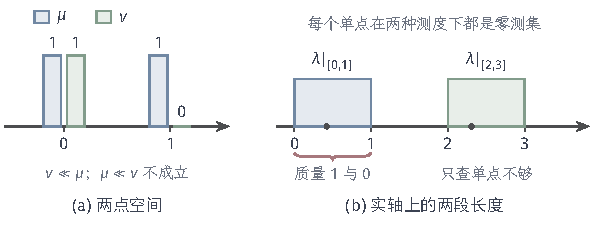
\includegraphics[width=100.669mm]{figures/02-abstract-mathematics/01-metric-and-measure/tikz/c2-absolute-continuity/figure.pdf}
  \caption{绝对连续比较的是零测集。(a)两点空间上$\mu=\delta_0+\delta_1$（蓝）与$\nu=\delta_0$（绿）：$\mu$只把空集看作零测集，所以$\nu\ll\mu$；$\nu$在点$1$的质量为零而$\mu$不为零，所以反向不成立。(b)$\lambda|_{[0,1]}$（蓝）与$\lambda|_{[2,3]}$（绿）在每个单点上都为零，但在$[0,1]$上分别为$1$与$0$，两者互不绝对连续。}
  \label{fig:measure-absolute-continuity}
\end{figure}

\paragraph{小质量控制}
“绝对连续”这个名字来自一个与函数连续性相似的说法：参考测度很小的集合，目标测度也很小。零测集的包含关系是“等于零推出等于零”，下面的定理把它加强为“接近零推出接近零”，但需要目标测度有限。

\begin{theorem}[绝对连续的小质量刻画]
\label{thm:measure-ac-epsilon-delta}
设$\mu,\nu$是$(X,\mathcal A)$上的非负测度，且$\nu$有限。则$\nu\ll\mu$当且仅当：对每个$\varepsilon>0$，存在$\delta>0$，使得对所有$A\in\mathcal A$，
\[
 \mu(A)<\delta\ \Longrightarrow\ \nu(A)<\varepsilon .
\]
\end{theorem}

\begin{proof}
先证充分性。设小质量条件成立，$\mu(A)=0$。对任意$\varepsilon>0$，取相应的$\delta$，则$\mu(A)=0<\delta$，故$\nu(A)<\varepsilon$。$\varepsilon$任意，所以$\nu(A)=0$。

再证必要性，用反证法。设$\nu\ll\mu$而小质量条件不成立，则存在某个$\varepsilon>0$，使得无论$\delta$取多小都有反例。依次取$\delta=2^{-n}$，得到可测集$A_n$满足
\[
 \mu(A_n)<2^{-n},\qquad \nu(A_n)\ge\varepsilon,\qquad n=1,2,\dots .
\]
这些集合的$\mu$质量趋于零，但$\nu$质量不趋于零。为了得到一个$\mu$零测而$\nu$质量为正的集合，考察尾并$B_k=\bigcup_{n\ge k}A_n$。由可数次可加性，
\[
 \mu(B_k)\le\sum_{n\ge k}2^{-n}=2^{1-k},
\]
同时$B_k\supseteq A_k$给出$\nu(B_k)\ge\varepsilon$。

尾并$B_1\supseteq B_2\supseteq\cdots$递减，令$B=\bigcap_kB_k$。对每个$k$有$\mu(B)\le\mu(B_k)\le2^{1-k}$，所以$\mu(B)=0$。另一方面，$\nu$有限，可以对递减集合列使用从上连续性（第~\ref{sec:measure-spaces-def}节），得$\nu(B)=\lim_k\nu(B_k)\ge\varepsilon>0$。这与$\nu\ll\mu$矛盾。
\end{proof}

证明中唯一用到$\nu$有限的地方是从上连续性。这个条件不能去掉。在$X=(0,1]$上取$I_k=(2^{-k},2^{1-k}]$，$k=1,2,\dots$，它们两两不交且并为$(0,1]$。令
\[
 \nu=\sum_{k=1}^\infty 2^k\lambda|_{I_k},\qquad\text{即}\quad \nu(A)=\sum_{k=1}^\infty 2^k\lambda(A\cap I_k),
\]
这是第~\ref{sec:measure-spaces-def}节中测度的可数加权和，仍是测度。若$\lambda(A)=0$，则每项$\lambda(A\cap I_k)=0$，所以$\nu(A)=0$，即$\nu\ll\lambda$。但$\lambda(I_k)=2^{-k}\to0$，而$\nu(I_k)=2^k\cdot2^{-k}=1$对每个$k$成立，小质量条件对$\varepsilon=1$失败。图~\ref{fig:measure-absolute-continuity-blocks}画出了前几块。这里$\nu((0,1])=\sum_k1=+\infty$，$\nu$不是有限测度，与定理并不矛盾。

\begin{figure}[!htbp]
  \centering
  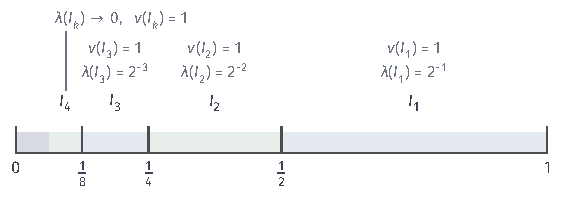
\includegraphics[width=95.324mm]{figures/02-abstract-mathematics/01-metric-and-measure/tikz/c2-absolute-continuity-blocks/figure.pdf}
  \caption{无限测度下小质量控制可能失败。$(0,1]$被分成$I_k=(2^{-k},2^{1-k}]$，它们的长度$\lambda(I_k)=2^{-k}$趋于零，而$\nu=\sum_k2^k\lambda|_{I_k}$给每块的质量都是$1$。$\nu\ll\lambda$成立，但长度小的集合不一定$\nu$质量小。}
  \label{fig:measure-absolute-continuity-blocks}
\end{figure}

\subsection{相互奇异}
\label{sec:measure-mutual-singularity}

绝对连续描述的是“一种测度忽略的地方，另一种也忽略”。与它相对的另一种极端是：两种质量各自待在对方忽略的区域里，互不重叠。

\paragraph{质量集中在不交的可测区域}
若$\nu(X\setminus N)=0$，就说$\nu$\emph{集中}在可测集$N$上：$N$之外没有$\nu$质量。两种测度可以分别集中在一个集合及其补集上。

\begin{definition}[相互奇异]
\label{def:measure-singular}
设$\mu,\nu$是$(X,\mathcal A)$上的非负测度。若存在$N\in\mathcal A$，使
\[
 \mu(N)=0,\qquad \nu(X\setminus N)=0,
\]
就称$\mu$与$\nu$\term{相互奇异}（mutually singular），记作$\mu\perp\nu$。
\end{definition}

定义里$\mu$与$\nu$的地位看似不同，实际是对称的：令$N'=X\setminus N$，则$\nu(N')=0$且$\mu(X\setminus N')=\mu(N)=0$，所以同一关系从$\nu$的角度看就是用补集$N'$作分割。直观地说，$X$被分成两个可测区域，$\nu$的全部质量在$N$中，$\mu$的全部质量在$N'$中。

最直接的例子是长度与点质量。在实轴上取$\mu=\lambda|_{[0,1]}$，$\nu=\tfrac12\delta_{1/2}$，令$N=\{1/2\}$，则$\mu(N)=0$，$\nu(\mathbb R\setminus N)=0$，所以$\mu\perp\nu$，见图~\ref{fig:measure-mutually-singular}(a)。注意点$1/2$恰好位于$[0,1]$的内部：相互奇异不要求两种质量在位置上分开，只要求存在一个可测集合把它们分开。

相互奇异与绝对连续几乎不能同时成立。若$\nu\ll\mu$且$\nu\perp\mu$，取定义中的$N$，则$\mu(N)=0$推出$\nu(N)=0$，再加上$\nu(X\setminus N)=0$，得$\nu(X)=0$，即$\nu$是零测度。这个简单事实将在第~\ref{sec:measure-decomposition}节证明分解唯一时用到。

\paragraph{可测分离不等于距离分离}
在实轴上，“相互奇异”很容易被想象成两团质量隔着一段距离。下面的例子说明这种想象不对。设$(q_n)_{n\ge1}$列举$\mathbb Q$中的全部有理数，令
\[
 \mu=\sum_{n=1}^\infty2^{-n}\delta_{q_n},\qquad
 \nu=\sum_{n=1}^\infty2^{-n}\delta_{q_n+\sqrt2},
\]
两者都是总质量为$\sum_n2^{-n}=1$的有限测度。$\mu$集中在$\mathbb Q$上，$\nu$集中在$\mathbb Q+\sqrt2=\{q+\sqrt2:q\in\mathbb Q\}$上。这两个集合不相交：若$q=q'+\sqrt2$，则$\sqrt2=q-q'$是有理数，矛盾。于是取$N=\mathbb Q+\sqrt2$，有$\mu(N)=0$，$\nu(\mathbb R\setminus N)=0$，$\mu\perp\nu$。

另一方面，$\mathbb Q$与$\mathbb Q+\sqrt2$都在实轴上稠密：每个非空开区间$(a,b)$中既有有理数$q_n$，也有形如$q_m+\sqrt2$的点（取$(a-\sqrt2,b-\sqrt2)$中的有理数$q_m$）。所以$\mu((a,b))\ge2^{-n}>0$且$\nu((a,b))\ge2^{-m}>0$，两种测度在每个非空开区间上都有正质量。图~\ref{fig:measure-mutually-singular}(b)画出了两组点中的前几个，它们彼此交错。可见相互奇异是可测集合层面的分离，与第~\ref{chap:metric-spaces}章的距离结构无关。顺带一提，$\mu$与$\nu$都集中在可数集上，而可数集是Lebesgue零测集，所以它们与$\lambda$也都相互奇异。

\begin{figure}[!htbp]
  \centering
  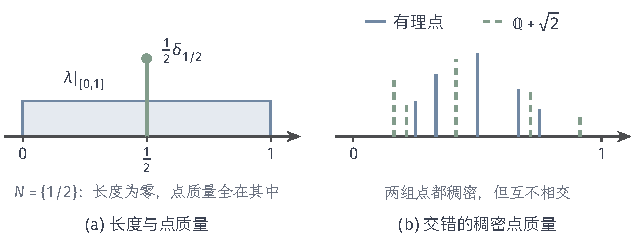
\includegraphics[width=107.668mm]{figures/02-abstract-mathematics/01-metric-and-measure/tikz/c2-mutually-singular/figure.pdf}
  \caption{相互奇异是可测集合上的分离。(a)$\lambda|_{[0,1]}$与$\tfrac12\delta_{1/2}$相互奇异，分离集$N=\{1/2\}$位于区间内部。(b)$\mu=\sum_n2^{-n}\delta_{q_n}$集中在有理点上（蓝色实线），$\nu=\sum_n2^{-n}\delta_{q_n+\sqrt2}$集中在$\mathbb Q+\sqrt2$上（绿色虚线）；图中只画出$[0,1]$内各几个点，线高仅示意权重递减。两组点在每个开区间中都出现，但互不相交，所以$\mu\perp\nu$。}
  \label{fig:measure-mutually-singular}
\end{figure}
